% !TEX root = thesis.tex
\graphicspath{ {./figures/} }

%%%%%%%%%%%%%%%%%%%%
\chapter{Evaluation}
%%%%%%%%%%%%%%%%%%%%

The three algorithms will be evaluated based on their runtime and scalability as well as their robustness, meaning their ability to handle invalid graphs. 

\section{Method}

We will explore the runtime of the algorithms on small graphs, big graphs and then explore their behavior in specific situations and corner cases. For the first two sections, we have built an algorithm, that builds a graph with n nodes, and then adds between zero and three delegations per node to random other nodes, ensuring that there are no delegation cycles without a sink. A better explanation of how these graphs are artificially constructed can be found in the Annex. \TODO{Create this annex} We acknowledge, that these assumptions may not be representative of real delegation graphs, where, as studies have shown, delegates tend to not delegate randomly, but to a subset of experts, such as TV personalities, thus centering power to one or few people. This approach also ignores potential tendencies such as friends delegating to eachother more likely. Such situations will be explored in subsection XX. \TODO{Add citations that these situations happen. Maybe the viscous democracy paper, and the pirate party example, and in one of the six original papers Ford shared this was also mentioned}.

To minimize the impact of background noise and measurement fluctuations on the benchmarks, algorithms with very short runtimes were executed multiple times, and the average runtime was recorded. The recorded runtimes always indicate just the runtime for the algorithms to resolve the delegations, times for set-up, such as the time for building the linear program, were not included. 

\section{Evaluating Runtime and Scalability}

\subsection{Small graphs}
\label{subsec:small_graphs}

\begin{figure}[h]
    \centering
    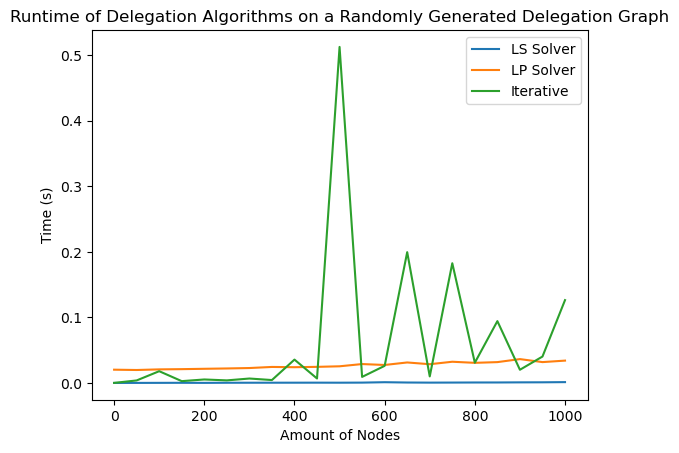
\includegraphics[width=0.4\textwidth]{0-1000_random}
    \caption{Runtime of delegation algorithms on a randomly generated delegation graph.}
    \label{fig:random-small}
\end{figure}

In order to explore the three algorithm's behavior on small graphs, we used the graph generator to generate graphs with zero to 1000 nodes. \Cref{fig:random-small} shows the results of this benchmark.

We can see, that the LS Implementation, optimized for sparse matrices, outperforms the other two algorithms. Its growth in runtime is so small, that the line looks to be staying flat on the x-axis. However, with a graph of 1000 nodes, its runtime is about 0.01 seconds. Both the LS and LP implementation display a rather steady, yet growing runtime. The LP solver seems to have some overhead, since even when the graph has zero nodes, it has a runtime of about 0.02 seconds.

Furthermore, we can interestingly observe large spikes in the runtime of the iterative approach. Exploring this more closely, we find that the graph with 11 nodes takes the iterative algorithm a lot more time than the graph with 10 or 12 nodes, as shown in \cref{fig:random-tiny}. At 10 nodes, the runtime of the iterative algorithm is just about 0.004 seconds, at 12 nodes it is 0.001 seconds, so even slightly faster than the slightly smaller graph, but when the graph has 11 nodes, the runtime skyrockets to about 0.056 seconds.

\begin{figure}[h]
    \centering
    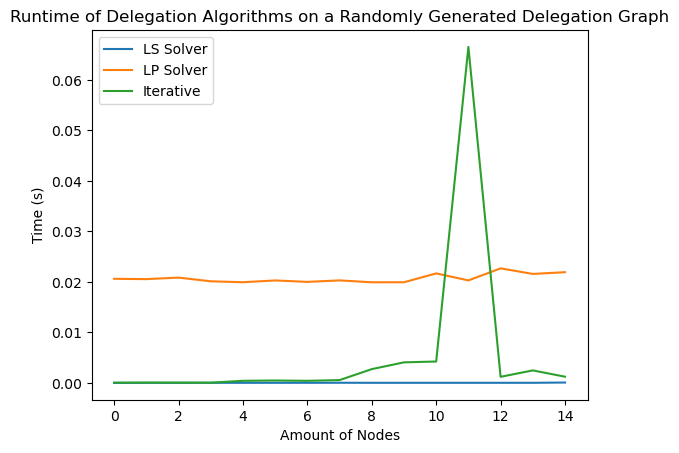
\includegraphics[width=0.4\textwidth]{0-15_random}
    \caption{Runtime of delegation algorithms on a randomly generated delegation graph.}
    \label{fig:random-tiny}
\end{figure}

A possible explanation for this spike may be, that when the graph has 10 and 12 nodes, it iterates only 758 and 170 times respectively, before cutting off, while when it has 11 nodes it iterates 8735 times before cutting off. \Cref{fig:random-11and12} shows the two graphs with 11 and 12 nodes.

\begin{figure}[h]
    \centering
    \begin{subfigure}[t]{0.45\textwidth}
        \centering
        \fbox{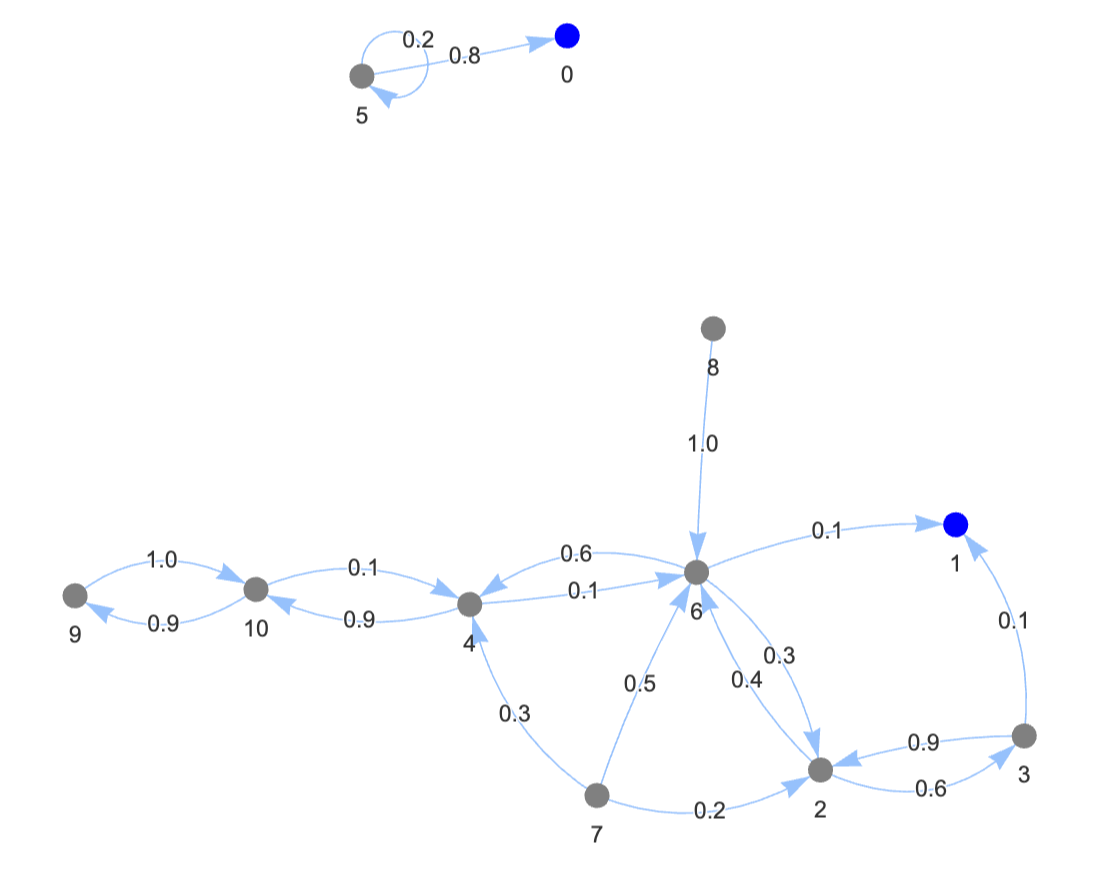
\includegraphics[width=\textwidth]{11_random}}
        \caption{11 nodes}
        \label{subfig:random-11and12-11}
    \end{subfigure}
    \hfill
    \begin{subfigure}[t]{0.45\textwidth}
        \centering
        \fbox{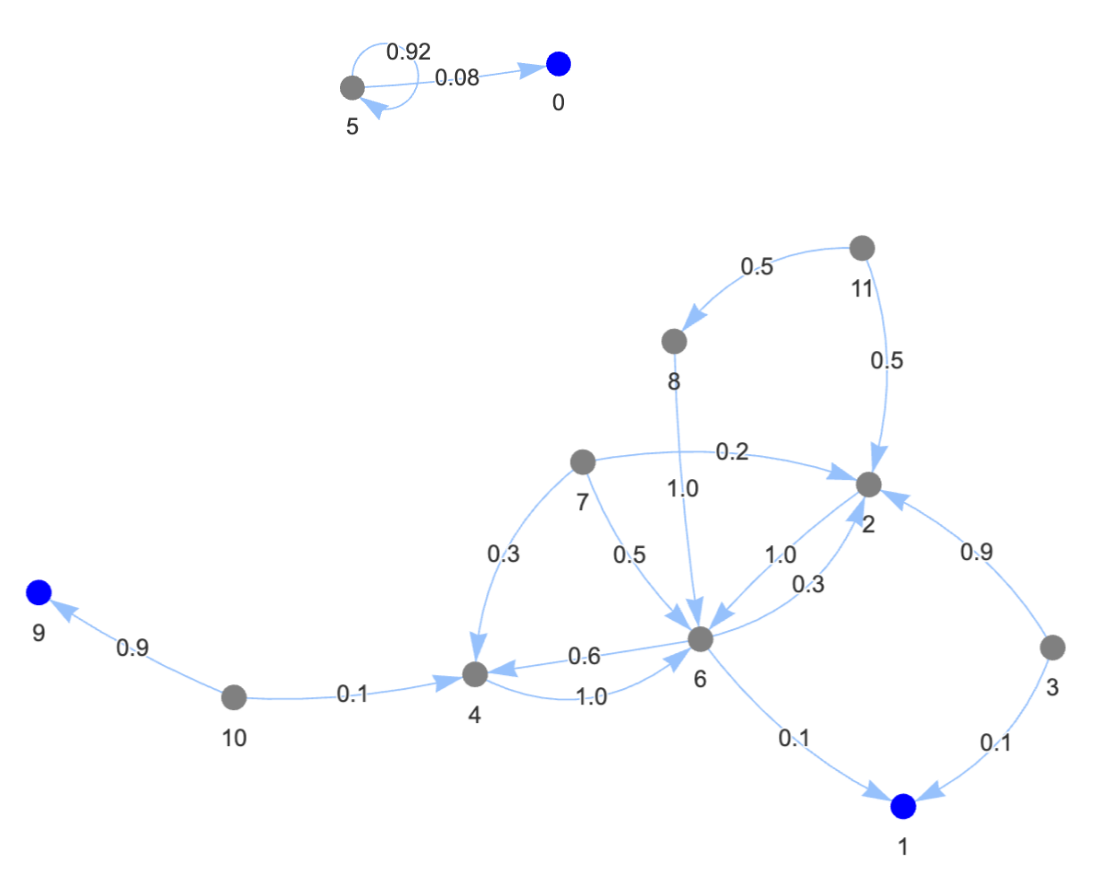
\includegraphics[width=\textwidth]{12_random}}
        \caption{12 nodes}
    \end{subfigure}
    \caption{Delegation graphs with 11 and 12 nodes}
    \label{fig:random-11and12}
\end{figure}

Inspecting the graphs reveals a possible explanation for this behavior. When the graph has 12 nodes, node \texttt{9} is a sink, while in the graph with 11 node it delegates its power back to node \texttt{10}. In the latter case, power going out of node \texttt{9} needs to pass to node \texttt{10}, \texttt{4} and \texttt{6} before reaching a sink. While passing through node \texttt{4}, we can see that 90\% of the power is delegated back into the cycle between nodes \texttt{4}, \texttt{10} and \texttt{9}. The algorithm will iterate power through this loop, until enough has been drained out for the \texttt{total\_change} to fall below the cutoff. 

This is an important shortcoming of the iterative algorithm. Power can easily get trapped within permissible delegation cycles that only have a small drain allowing the power to escape from the cycle. Each iteration, if a great proportion of the nodes with draining edges' power is sent back into a cycle, the algorithm needs to continuously iterate until the power is back at the drain nodes, however depending on the cycle this may happen very inefficiently. This phenomenon will be tested more in \cref{subsec:cycles_draining}

\subsection{Large Graphs}

Delegation graphs may grow arbitrarily large. National elections for example can contains up to hundreds of millions of participants. This section explores how the algorithms perform when having to resolve graphs with a lot of nodes. Again, the graphs will be randomly generated, such that each nodes has between 0 and 3 delegates. 

\begin{figure}[h]
    \centering
    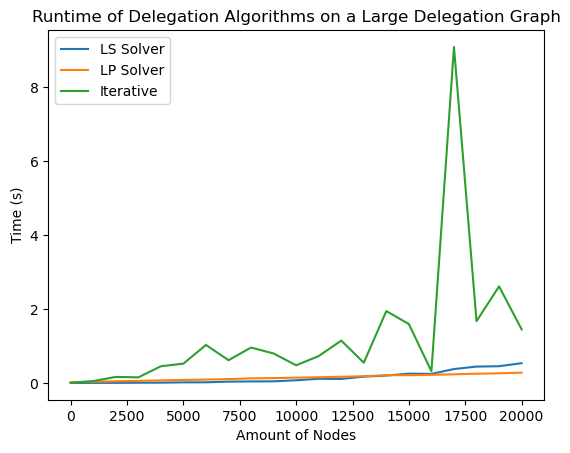
\includegraphics[width=0.4\textwidth]{0-20000_random}
    \caption{Runtime of delegation algorithms on a randomly generated delegation graph.}
    \label{fig:random-large}
\end{figure}

In \cref{fig:random-large} we can see, that it is difficult to determine a pattern in the runtime for the iterative algorithm. Depending on the underlying delegation graph, the runtime can grow unpredictably large. What is evident from the runtime graph however, is that in as the graphs get larger its runtime never subceeds the runtimes of the other two algorithms, while it is worth mentioning that for some graphs, the iterative algorithm's runtime is not a lot longer than that of the other two algorithms. It is difficult to make any statement about the runtime class of the iterative algorithm based just on the number of nodes in the graph, since, depending on the structure of the graph and the cutoff value the runtime can get arbitrarily high. The comparatively high runtime of the iterative algorithm overshadows the runtimes of the other two, so in order to better discuss and analyze their performance, \cref{fig:random-large-no-iterative} shows the same graph as in \cref{fig:random-large}, without the runtimes for the iterative algorithm.

\begin{figure}[h]
    \centering
    \begin{subfigure}[t]{0.45\textwidth}
        \centering
        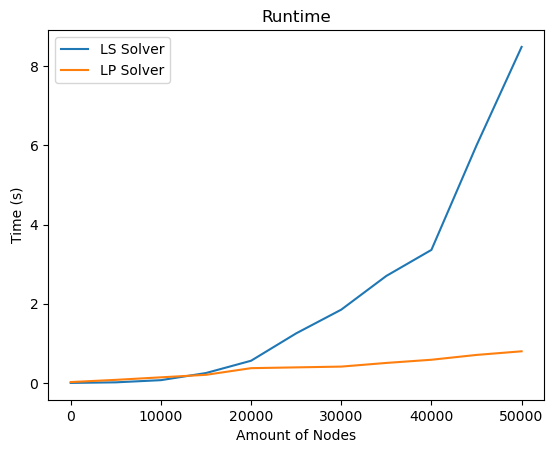
\includegraphics[width=\textwidth]{0-50000_random_no_iterative}
        \caption{Linear scale}
         \label{subfig:random-large-no-iterative-linear}
    \end{subfigure}
    \hfill
    \begin{subfigure}[t]{0.45\textwidth}
        \centering
        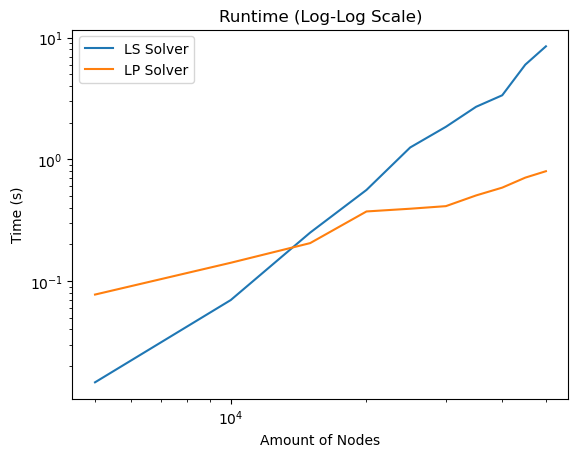
\includegraphics[width=\textwidth]{0-50000_random_no_iterative_loglog}
        \caption{Loglog scale}
         \label{subfig:random-large-no-iterative-loglog}
    \end{subfigure}
    \caption{Runtime of delegation algorithms on a randomly generated delegation graph.}
    \label{fig:random-large-no-iterative}
\end{figure}

\begin{figure}[h]
    \centering
    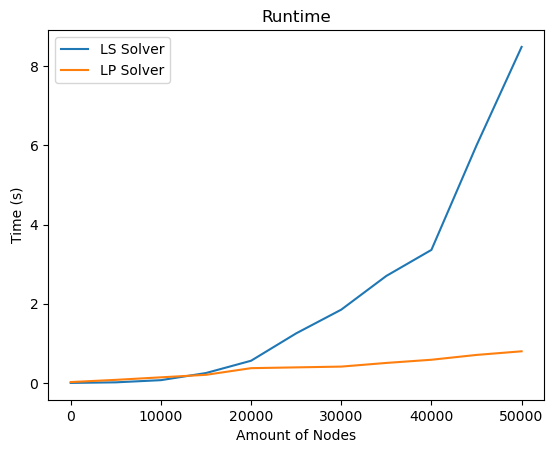
\includegraphics[width=0.4\textwidth]{0-50000_random_no_iterative}
    \caption{Runtime of delegation algorithms on a randomly generated delegation graph.}
    \label{fig:random-large-no-iterative}
\end{figure}

\Cref{subfig:random-large-no-iterative-linear} shows, that as the delegation graph grows, the LP solver's runtime grows more slowly than the LS Solver's. For resolving smaller graphs, the LS solver outperforms the LP solver, with a runtime of almost zero for empty or very small graphs, while the LP solver has a clearly non-zero runtime even for very small graphs. However, at around 12 000 nodes, this changes, as the LP solver's runtime's slower growth catches up with that of the LS solver. 

The type of growth, so the runtime class, is not immediately clear from the graphs, although the LP solver's growth seems to be more linear than that of the LS solver. Looking at the same results on a loglog graph reveals, that the LS solvers runtime may follow a power law.

Fitting the data into different kinds of curves reveals, that the LP implementations runtime likely has linear growth, while the LS solver grows following a power distribution, such that it is in the runtime class of $O(n^{2.778})$.

\TODO{Put the runtime results and/or the code and the regression results into the annex, or into the text...}

\subsection{Dense Graphs}

While we expect most delegators in any delegation graph to only delegate to a handful of people, a well formed delegation graph can have any number of delegates per delegator. Thus, it is also interesting to compare how the three algorithms compare when resolving more dense graphs. In this section, we test the three implementations on NetworkX's $G_{n,p}$ graph generator \texttt{gnp\_random\_graph}, which returns a directed graph with $n$ nodes, where each node connected to each other node with probability $p$, which is set to $0.5$ for the remainder of this section.\TODO{Insert missing citation} These graphs are not well-formed delegation graphs out-of-the box, thus we adapt them by removing outgoing edges of nodes, turning them into sinks, until 10\% of the nodes are sinks. Then, each delegators vote is equally distributed to all of its outgoing edges, such that the edge weights add up to 1. Finally, any closed delegation cycles are removed by removing a random edge in the cycle (and re-normalizing the edge weights). 

% \TODO{cite here https://networkx.org/documentation/stable/reference/generated networkx.generators.random_graphs.gnp_random_graph.html} at the end of the sentence where I introduce this graph

\begin{figure}[h]
    \centering
    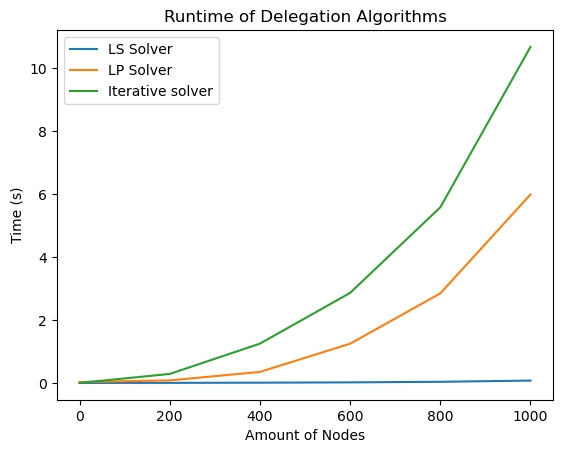
\includegraphics[width=0.4\textwidth]{0-1000_dense}
    \caption{Runtime of delegation algorithms on a randomly generated delegation graph.}
    \label{fig:dense-small}
\end{figure}

\Cref{fig:dense-small} shows the runtime of these three algorithms. The runtime of the iterative algorithm lacks the spikes found when resolving sparse graphs. This is likely due to the nature of the graphs we create. Every delegator is connected to half of all other nodes ($p = 0.5$), and of these $10\%$ are sinks, thus power drains quickly into sinks, and situations where power iterates a long time without seeing a sink are less frequent. Regardless, the iterative algorithm exhibits the worst runtime of the three. 

\begin{figure}[h]
    \centering
    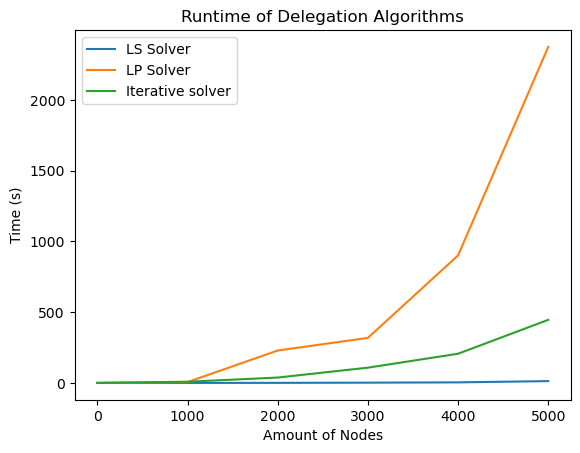
\includegraphics[width=0.4\textwidth]{0-5000_dense}
    \caption{Runtime of delegation algorithms on a randomly generated delegation graph.}
    \label{fig:dense-large}
\end{figure}

Testing the three algorithms on larger dense graphs, reveals surprisingly, that the LP solver's runtime is considerably worse than that of both the iterative and LS solver. A dense graph with 5,000 nodes, and thus about 125,000 delegations, takes the LS solver only about 12 seconds, the iterative solver 445 seconds, and the LP solver almost 2,400 seconds. Even though the LS solver is optimized for sparse matrices, it outperforms the other two implementations on dense graphs.


\subsection{Cycles which Retain a Lot of their Power}
\label{subsec:cycles_draining}

\begin{figure}[h]
	\centering
	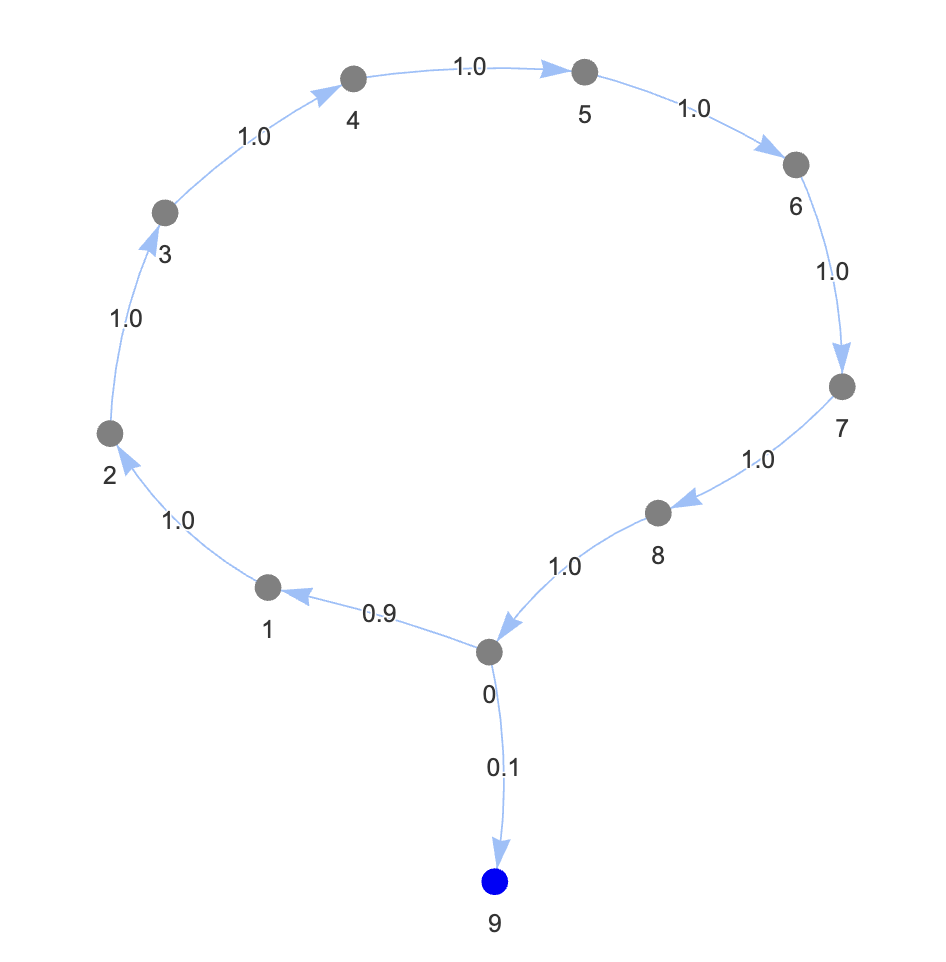
\includegraphics[width=0.4\textwidth]{big_cycle_example}
	\caption{An example of the cycles used for the benchmarks. The blue node is the sink}
	\label{fig:big_cycle_example}
\end{figure}

To further explore one of the iterative algorithm's shortcomings, this section will explore and compare runtime behavior for delegation cycles which are not closed, but contain only few, weak edges for power to drain, thus forcing power to iterate around in the cycle before it reaches a sink. Specifically, we construct graphs with delegates all delegating power to the next node in the cycle. One node in the cycle contains an edge with weight 0.1 to a sink, while the other 0.9 of its power go to the first node in the cycle. \Cref{fig:big_cycle_example} contains an exemplary image of such a graph with 10 nodes. 

\begin{figure}[h]
    \centering
    \begin{subfigure}[t]{0.45\textwidth}
    	\centering
    	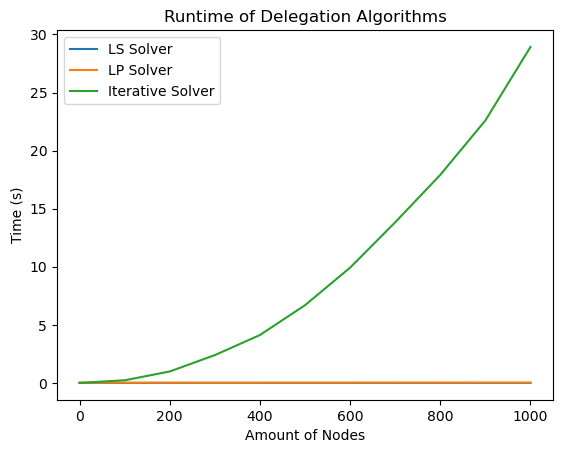
\includegraphics[width=\textwidth]{0-1000_cycle}
    	\caption{Linear scale}
    	\label{subfig:cycle-small-linear}
    \end{subfigure}
    \hfill
    \begin{subfigure}[t]{0.45\textwidth}
        \centering
        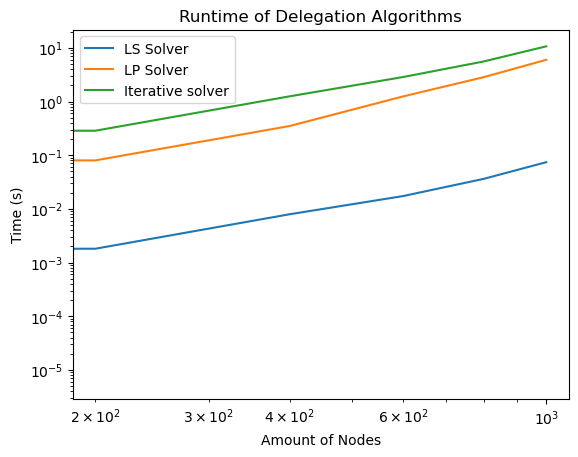
\includegraphics[width=\textwidth]{0-1000_dense_loglog}
        \caption{Loglog scale}
         \label{subfig:cycle-small-loglog}
    \end{subfigure}
    \caption{Runtime of delegation algorithms on a randomly generated delegation graph.}
    \label{fig:cycle_small}
\end{figure}

The runtimes in \cref{subfig:cycle-small-linear} show, that as expected, the iterative algorithm struggles considerably with the resolution of these graphs, while the other two algorithms exhibit behavior similar to that on randomly generated sparse delegation graphs. The growth of the runtimes seems to be polynomial, with the iterative algorithm belonging to the runtime class $O(n^{2.12})$. Being able to resolve these kinds of loops is one of the greatest strength of the two approaches, which don't simulate power as flow through the graph. By directly solving the system of linear equations, they are a lot more well equipped to deal with this specific corner case.  

\begin{figure}[t]
	\centering
    	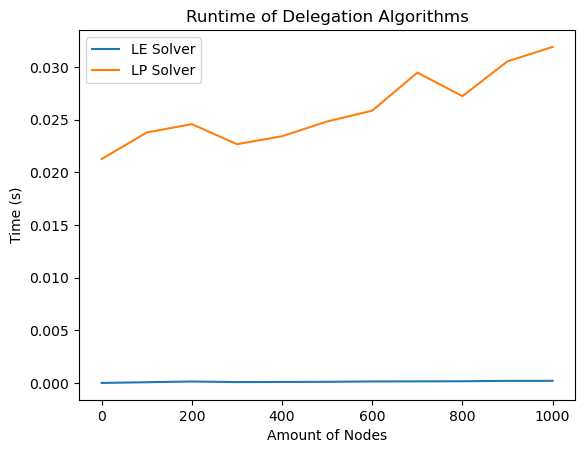
\includegraphics[width=0.4\textwidth]{0-1000_cycle_no_iterative}
    	\caption{Runtime of delegation algorithms on a randomly generated delegation graph.}
	\label{fig:cycle-small-no-iterative-linear}
\end{figure}

As seen in \cref{fig:cycle-small-no-iterative-linear}, which shows the same graph as in \cref{subfig:cycle-small-linear} without the iterative algorithm's runtime, the runtime of the LS and LP Solvers grows similarly to when resolving randomly generated (sparse) delegation graphs, such as the ones found in \cref{subsec:small_graphs}.

Such a cycle as the one we deliberately constructed is not the only situation in which the iterative algorithm will struggle. As long as power is not efficiently funneled toward a sink, the iterative algorithm will have to spend more time moving the power around until enough has drained into a sink for \texttt{total\_change} to fall below the cutoff value. A further example of such behavior is the cycle that caused runtime to spike in \cref{subfig:random-11and12-11}. An artificial example of this situation is shown below in Figure XX. \TODO{Create this graph}


\subsection{Real Example}

So far, we have made use mainly of randomly or artificially generated graphs. This section will briefly confirm, that our insights also hold when resolving delegations based on 

\TODO{I want to try the algorithm on one huge, "real" dataset here}

\TODO{Standord's Large Network Dataset Collection "Epinions" dataset is cool.} 

\TODO{Ill do this later, since while its a cool addition, its probably not going to add a lot of insight thats necessary for the first draft...}


\section{Robustness}

This section the different implementations behavior when a delegation graph is not well formed. Specifically, their behaviors when outgoing delegation weights are invalid, so not adding up to 1, and if the delegation graph contains a closed delegation cycle. 

\subsection{Invalid delegations}

On their own, neither of the three implementations will definitively cause an error when delegations are invalid. The iterative implementation is "dumb", in the sense that it moves around power as it finds them in the delegations. If a delegator delegates more than they are meant to, the algorithm behavior becomes undefined, since the delegators power may become negative, at which point the delta in power calculated from its power also becomes negative, which messes with the \texttt{total\_change} value in unpredictable ways. 

If a delegate delegates less than their vote, this causes less of an issue. As long as the delta calculated at $\delta \gets w \times \texttt{prev\_powers}[u]$ does not become negative, the algorithm's behavior becomes quite predictable. A well-formed delegation graph is allowed to contain self-delegations as long as their weight is lower than 1, such as the delegation in \cref{subfig:permissible-self-delegation}. In this situation, power still leaves the node, but less slowly. When the iterative algorithm goes over the graph, not delegating enough weight has the same effect as such a self-delegation, since in the former situation  power gets subtracted and then re-added to the node, while in the latter it just remains untouched.

\begin{figure}[h]
    \centering
    \begin{subfigure}[t]{0.45\textwidth}
	\centering
	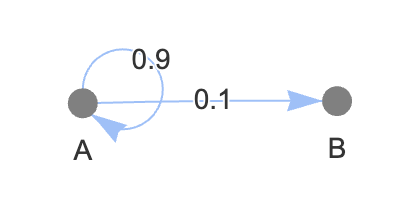
\includegraphics[width=0.9\textwidth]{allowed_self_loop}
	\caption{Permissible delegation graph}
	\label{subfig:permissible-self-delegation}
    \end{subfigure}
    \hfill
    \begin{subfigure}[t]{0.45\textwidth}
        \centering
        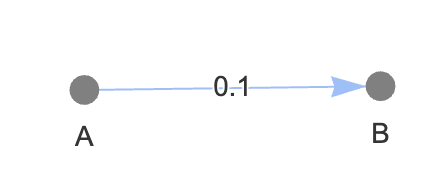
\includegraphics[width=\textwidth]{invalid_delegation_graph}
        \caption{Invalid delegation graph}
         \label{subfig:invalid-delegation-graph}
    \end{subfigure}
    \caption{Two similar delegation graphs}
    \label{fig:small-delegation-graphs}
\end{figure}

For the two implementations based on systems of linear equations, this is a little different. Node \texttt{B}'s power would end up as 1.1, since the system of linear equations looks as follows:

\begin{align*}
& p_A = 1 \\
& p_B = 1 + 0.1p_A
\end{align*}

As long as the delegations form a matrix that is singular, there will be a unique solution, so even with invalid delegations, the algorithm will find power values, however they most likely not conserve power properly. 

\subsection{Closed Delegation Cycles}

If the delegations form a closed delegation cycle, the iterative algorithm will not terminate, since the algorithm will iterate any power that is in or enters the cycle around the cycle indefinitely. 

For the other two algorithms however, such a cycle can be caught. The equations for the standing power of the nodes within the cycle are linearly dependent on each other, thus the matrix resulting from them is not singular, and hence don't have a single solution. Solvers of systems of linear equations catch and throw an error.

What is worth mentioning however, is that since we allow fractional delegation, it suffices if just one node is a closed delegation cycle does also delegates to a node outside of a delegation cycle (or turns into a sink), for the delegations to become resolvable again. The cycles that were explored in \cref{subsec:cycles_draining} are example of such a situation. While closed delegation loops frequently pose a problem in liquid democracies \TODO{cite}, they happen less frequently when allowing fractional delegation \TODO{cite}.



%TODO Maybe mention also at some point, that this evaluation is a comparison between different solvers for systems of linear equations